\section{目的}
依據所提供 \textit{DIC Lab.pdf} 的 Lab 1（PDF 第 3--9 頁），重新建立 NMOS 與 PMOS 的直流特性實驗，逐項完成四個實驗步驟與四個討論問題。目的包括辨識二極體接法的轉移曲線、比較不同閘極偏壓的輸出曲線、量化通道長度對輸出斜率的影響，以及分析弱反轉區的半對數斜率。

本版為使用由使用者另行提供的模型庫所作的教學改寫。講義曲線使用舊製程及最高 2.5--4 V 的偏壓；本版將端點電壓的絕對值限制在 1.0 V 範圍進行比較，並保留講義的基本尺寸。1.0 V 是本次選定的模擬條件，不是由加密模型驗證的安全額定。新結果不宣稱重現原製程的數值或崩潰區。

\section{Spec 對照}
下表以講義的實驗步驟和問題為驗收單位；「已模擬」只代表所列的本次模擬條件成功執行，並不等於原製程數值已重現。
\begin{center}
\setlength{\tabcolsep}{3pt}
\begin{tabular}{p{0.42\linewidth}p{0.29\linewidth}p{0.23\linewidth}}
\toprule
規格（PDF 頁） & 實作檔案 & 核對狀態 \\
\midrule
步驟 1：二極體接法 $I_D$--$V_{GS}$（8） & \texttt{01\_diode\_n/p.sp} & 已模擬；本次偏壓 \\
步驟 2：分開 G/D，多組閘壓（8） & \texttt{02\_output\_n/p.sp} & 已模擬；本次範圍 \\
步驟 3：固定 W，改變 L（8） & \texttt{03\_length.sp} & 已模擬；改變偏壓 \\
步驟 4：弱反轉半對數曲線（8） & \texttt{04\_subthreshold.sp} & 已擬合；區間限定 \\
問題 1：W/L 增加（9） & \texttt{01\_diode\_n/p.sp} & 三種 W 已比較 \\
問題 2：等 W/L 的 N/P 電流比（9） & \texttt{05\_equal\_geometry.sp} & 已量測；非遷移率 \\
問題 3：飽和區斜率與 L（9） & \texttt{03\_length.sp} & 已量測區間割線 \\
問題 4：弱反轉斜率比較（9） & \texttt{04\_subthreshold.sp} & 已量測近似斜率 \\
\bottomrule
\end{tabular}
\end{center}

\section{電路與設計推導}
步驟 1 依圖 1.2(a) 將 Gate 與 Drain 短接，而非固定 $V_{DS}$ 掃 $V_{GS}$。這是對原始參考程式的重要修正。步驟 2 才將兩端分開，由獨立電壓源設定 Gate 與 Drain。NMOS 的 Source/Bulk 均接 0；PMOS 的 Source/Bulk 也接 0，Gate/Drain 使用負偏壓，確保 $V_{SG},V_{SD}$ 的幅值可直接與 NMOS 比較。

基準尺寸為 $W_n=0.6\,\mu\mathrm m$、$W_p=1.8\,\mu\mathrm m$、$L=0.25\,\mu\mathrm m$。模型名稱使用 \texttt{nmos/pmos}，未將通道長度一律改為 90 nm。MOS 元件一律明寫 \texttt{W=} 和 \texttt{L=}，PMOS 遞減掃描使用負步長。

長通道近似可寫成
\[
 I_D\simeq\frac{\mu C_{ox}}{2}\frac WL(V_{GS}-V_T)^2(1+\lambda V_{DS}).
\]
因此增加 W 通常使電流增加；縮小 L 不只改變 $W/L$，也可能改變短通道效應。此式用於解釋趨勢，計算數值仍採本次模型。輸出斜率使用 0.8--1.0 V 的割線
\[
g_{ds,\mathrm{sec}}=\frac{|I_D(1.0)|-|I_D(0.8)|}{0.2},
\]
不可將它直接當成 $\lambda$。半對數區域則定義
\[
S=\left(\frac{d\log_{10}|I_D|}{d|V_{GS}|}\right)^{-1},
\]
其單位為 V/dec；S 越大，半對數圖上的電流斜率越小。

\section{模擬設定}
使用 PrimeSim HSPICE S-2021.09 win64、25\,$^\circ$C，公開 deck 以註記保留模型設定位置；本機執行副本才載入另行提供的模型。七份獨立 \texttt{.sp} 可在模擬器中個別開啟；\texttt{.alter} 產生同一電路的參數比較。各檔輸出 \texttt{.sw*} 波形、\texttt{.ms*} 量測與 \texttt{.lis} 列印資料。

\begin{itemize}
\item 二極體接法：$|V_{GS}|=|V_{DS}|=0$--1 V、步距 1 mV；W 為基準的 1、2、4 倍。
\item 輸出曲線：$|V_{DS}|=0$--1 V、步距 1 mV；$|V_{GS}|=0,0.2,0.4,0.6,0.8,1.0$ V。
\item 長度比較：$L=0.25,0.50,0.75,1.00\,\mu\mathrm m$，W 固定，兩極性均取 $|V_{GS}|=0.6$ V。此偏壓與講義的 NMOS 1.6 V／PMOS 0.9 V 不同，故僅驗證本次模型下的同類趨勢。
\item 弱反轉曲線：$|V_{GS}|=0$--0.5 V；$|V_{DS}|=1.0,0.6,0.3$ V。只用 0.15--0.25 V 區間做線性擬合，不把全部掃描點都稱為弱反轉。
\item 等幾何比較：N/P 均為 $W/L=0.6/0.25\,\mu\mathrm m$，$|V_{DS}|=0.8$ V，在 $|V_{GS}|=0.8$ V 量測比值。
\end{itemize}
\texttt{.measure} 輸出的是波形上的指定量測數值，不能代替整條曲線。圖表由本次 HSPICE 的列印資料轉為 CSV 後重繪，來源可追溯至 \texttt{validation/dic\_pilot/}；電壓源電流符號與元件 Drain 電流相反，表格使用絕對值。

HSPICE 亦回報加密區塊的警告遭隱藏；以 \texttt{WARNLIMIT=100} 診斷仍無詳細訊息，因此不宣稱模擬為零警告。診斷量測與原結果一致，但不能據此判定警告無害。

\section{結果與規格檢查}
七份 deck 的所有分析均正常結束，未出現 \texttt{**error**} 或失敗的量測。二極體接法在 $|V_{GS}|=1.0$ V 的實際電流如下：
\begin{center}
\setlength{\tabcolsep}{3pt}
\begin{tabular}{lrr}
\toprule
W 倍數 & $|I_{Dn}|$ ($\mu$A) & $|I_{Dp}|$ ($\mu$A) \\
\midrule
1 & 198.491 & 112.529 \\
2 & 399.898 & 225.674 \\
4 & 802.707 & 451.963 \\
\bottomrule
\end{tabular}
\end{center}

電流接近隨 W 成正比，但並非精確整數倍。等幾何、$|V_{GS}|=|V_{DS}|=0.8$ V 時，NMOS 電流為 111.7734\,$\mu$A，PMOS 為 20.4637\,$\mu$A，比值為 0.183082。
\begin{figure}[htbp]
\centering
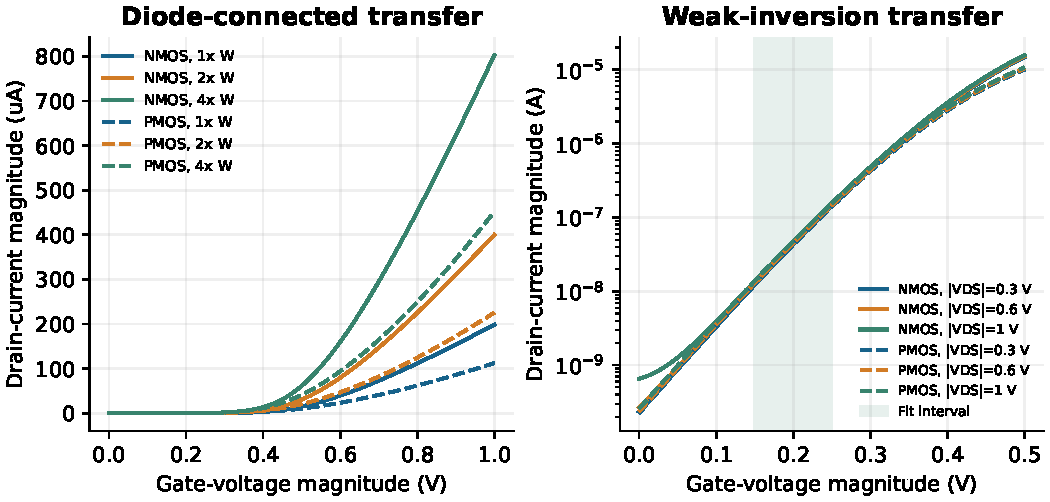
\includegraphics[width=\linewidth]{figures/dic01_characteristics.pdf}
\caption{本次 HSPICE 真實資料重繪的二極體接法與半對數轉移曲線；不是 WaveView 截圖。弱反轉斜率僅在文中指定區間擬合。}
\end{figure}
\begin{figure}[htbp]
\centering
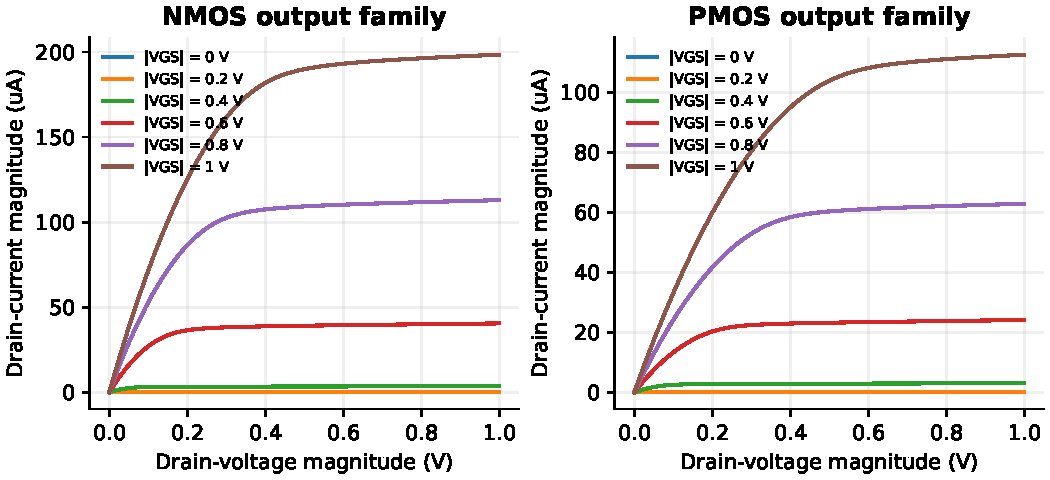
\includegraphics[width=\linewidth]{figures/dic01_output.pdf}
\caption{本次 HSPICE 資料重繪的 NMOS 與 PMOS 輸出特性族線；每條曲線對應一組固定閘極偏壓，Drain 電壓與電流均以幅值比較。}
\end{figure}

固定 $|V_{GS}|=0.6$ V，0.8--1.0 V 的輸出割線斜率如下。兩極性均隨 L 增加而下降。
\begin{center}
\setlength{\tabcolsep}{3pt}
\begin{tabular}{lrr}
\toprule
$L$ ($\mu$m) & $g_{ds,n}$ ($\mu$S) & $g_{ds,p}$ ($\mu$S) \\
\midrule
0.25 & 2.4410 & 1.6097 \\
0.50 & 0.6447 & 0.3574 \\
0.75 & 0.3445 & 0.1795 \\
1.00 & 0.2261 & 0.1141 \\
\bottomrule
\end{tabular}
\end{center}
\begin{figure}[htbp]
\centering
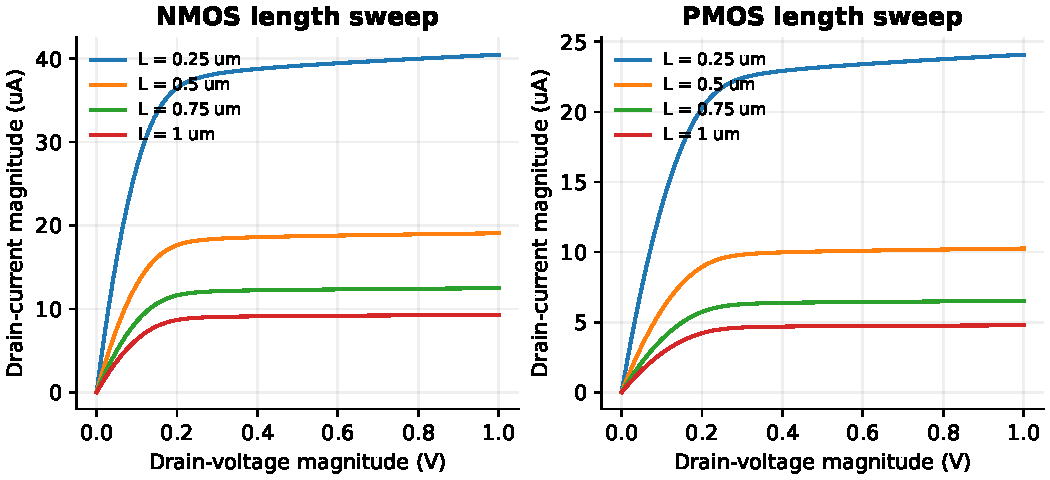
\includegraphics[width=\linewidth]{figures/dic01_length.pdf}
\caption{本次 HSPICE 資料重繪的 NMOS／PMOS 長度比較；固定 W 和閘極偏壓，圖中各曲線的 L 明確標示。}
\end{figure}

0.15--0.25 V 的半對數擬合結果如下：
\begin{center}
\setlength{\tabcolsep}{3pt}
\begin{tabular}{lrrrr}
\toprule
$|V_{DS}|$ (V) & $S_n$ (mV/dec) & $S_p$ (mV/dec) & $R_n^2$ & $R_p^2$ \\
\midrule
1.0 & 94.09 & 95.33 & 0.999865 & 0.999784 \\
0.6 & 93.65 & 95.13 & 0.999837 & 0.999789 \\
0.3 & 93.55 & 94.99 & 0.999837 & 0.999793 \\
\bottomrule
\end{tabular}
\end{center}

在 $|V_{DS}|=1$ V，區間內局部 S 約為 NMOS 91.06--99.11 mV/dec、PMOS 90.44--101.00 mV/dec。高 $R^2$ 支持此區間接近指數電流關係；本版未另外讀出模型的 $V_T$ 或 region 指標，因此將它記為「弱反轉區近似擬合」，不宣稱每個點皆由模型內部指標確認低於閾值。

\section{討論}
\textbf{問題 1：}本次固定 L、增加 W，電流約成比例增加，符合一階 $W/L$ 推導。改變 L 不能只靠同一比例預測，因為有效長度、寄生及短通道效應可能同時改變。

\textbf{問題 2：}相同 W/L 並不保證 $|I_{Dp}|/I_{Dn}=\mu_p/\mu_n$。即使使用平方律，也還需要相同的過驅動電壓和其他參數；本次模型的閾值、遷移率退化及速度飽和等因素均可能影響電流。量得的 0.183082 是這一偏壓下的電流比，不能當成加密模型的遷移率比。

\textbf{問題 3：}L 由 0.25 增至 1.00\,$\mu$m 時，兩極性的輸出斜率皆下降，顯示電流對 Drain 偏壓變化較不敏感。這與通道長度調變的定性推導一致，但本報告沒有用單一割線抽取 $\lambda$。

\textbf{問題 4：}以 $|V_{GS}|$ 為橫軸比較，本次 1 V Drain 偏壓下 PMOS 的擬合 S 略大，等價於半對數電流斜率略小。局部 S 隨 Gate 偏壓改變，N/P 的局部範圍也重疊，因此這不是所有偏壓或製程下的普遍排序。其差異需由各元件的電容耦合、次臨界因子及模型參數解釋；加密模型不提供本次可直接驗證的個別參數值。

\section{結論}
四個實驗步驟與四個問題均有對應程式、實際 HSPICE 資料及討論；已修正原始程式的二極體接法缺失與 PMOS 掃描方向。結果支持寬度增加使電流增大、長度增加使輸出斜率減小，以及指定區間近似指數導通的觀察。驗收範圍為所列的本次模擬條件；原製程的高電壓曲線、崩潰特性與模型閾值內部狀態不屬於已驗證結果。
